\chapter{Cartesian Coordinates}



\section{Grids}

The following code allows for the creation of \autoref{fig:grid1} and \autoref{fig:grid2}

\begin{verbatim}
\makeatletter
\def\grd@save@target#1{%
  \def\grd@target{#1}}
\def\grd@save@start#1{%
  \def\grd@start{#1}}
\tikzset{
  grid with coordinates/.style={
    to path={%
      \pgfextra{%

        \edef\grd@@target{(\tikztotarget)}%
        \tikz@scan@one@point\grd@save@target\grd@@target\relax
        \edef\grd@@start{(\tikztostart)}%
        \tikz@scan@one@point\grd@save@start\grd@@start\relax

       \draw[minor help lines] (\tikztostart) grid (\tikztotarget);

        \draw[major help lines] (\tikztostart) grid (\tikztotarget);

        \grd@start

        \pgfmathsetmacro{\grd@xa}{\the\pgf@x/1cm}
        \pgfmathsetmacro{\grd@ya}{\the\pgf@y/1cm}

        \grd@target

        \pgfmathsetmacro{\grd@xb}{\the\pgf@x/1cm}
        \pgfmathsetmacro{\grd@yb}{\the\pgf@y/1cm}

        \pgfmathsetmacro{\grd@xc}{\grd@xa + \pgfkeysvalueof{/tikz/grid with coordinates/major step}}

        \pgfmathsetmacro{\grd@yc}{\grd@ya + \pgfkeysvalueof{/tikz/grid with coordinates/major step}}

        \foreach \x in {\grd@xa,\grd@xc,...,\grd@xb}
        \node[anchor=north] at (\x,\grd@ya) {\pgfmathprintnumber{\x}};

        \foreach \y in {\grd@ya,\grd@yc,...,\grd@yb}
        \node[anchor=east] at (\grd@xa,\y) {\pgfmathprintnumber{\y}};
      }
    }
  },
  minor help lines/.style={
    help lines,
    step=\pgfkeysvalueof{/tikz/grid with coordinates/minor step}
  },
  major help lines/.style={
    help lines,
    line width=\pgfkeysvalueof{/tikz/grid with coordinates/major line width},
    step=\pgfkeysvalueof{/tikz/grid with coordinates/major step}
  },
  grid with coordinates/.cd,
  minor step/.initial=.2,
  major step/.initial=1,
  major line width/.initial=2pt,
}
\makeatother
\end{verbatim}

\makeatletter
\def\grd@save@target#1{%
  \def\grd@target{#1}}
\def\grd@save@start#1{%
  \def\grd@start{#1}}
\tikzset{
  grid with coordinates/.style={
    to path={%
      \pgfextra{%

        \edef\grd@@target{(\tikztotarget)}%
        \tikz@scan@one@point\grd@save@target\grd@@target\relax
        \edef\grd@@start{(\tikztostart)}%
        \tikz@scan@one@point\grd@save@start\grd@@start\relax

       \draw[minor help lines] (\tikztostart) grid (\tikztotarget);

        \draw[major help lines] (\tikztostart) grid (\tikztotarget);

        \grd@start

        \pgfmathsetmacro{\grd@xa}{\the\pgf@x/1cm}
        \pgfmathsetmacro{\grd@ya}{\the\pgf@y/1cm}

        \grd@target

        \pgfmathsetmacro{\grd@xb}{\the\pgf@x/1cm}
        \pgfmathsetmacro{\grd@yb}{\the\pgf@y/1cm}

        \pgfmathsetmacro{\grd@xc}{\grd@xa + \pgfkeysvalueof{/tikz/grid with coordinates/major step}}

        \pgfmathsetmacro{\grd@yc}{\grd@ya + \pgfkeysvalueof{/tikz/grid with coordinates/major step}}

        \foreach \x in {\grd@xa,\grd@xc,...,\grd@xb}
        \node[anchor=north] at (\x,\grd@ya) {\pgfmathprintnumber{\x}};

        \foreach \y in {\grd@ya,\grd@yc,...,\grd@yb}
        \node[anchor=east] at (\grd@xa,\y) {\pgfmathprintnumber{\y}};
      }
    }
  },
  minor help lines/.style={
    help lines,
    step=\pgfkeysvalueof{/tikz/grid with coordinates/minor step}
  },
  major help lines/.style={
    help lines,
    line width=\pgfkeysvalueof{/tikz/grid with coordinates/major line width},
    step=\pgfkeysvalueof{/tikz/grid with coordinates/major step}
  },
  grid with coordinates/.cd,
  minor step/.initial=.2,
  major step/.initial=1,
  major line width/.initial=2pt,
}
\makeatother

The first example of grid construction generates \autoref{fig:grid1}.
\begin{verbatim}
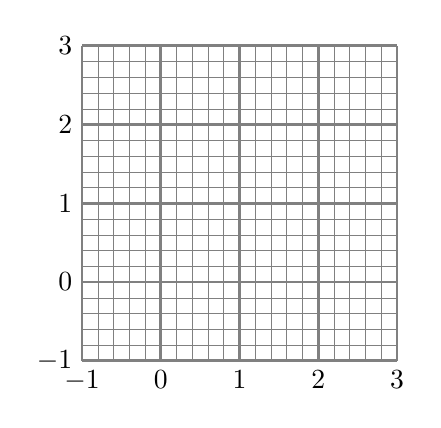
\begin{tikzpicture}

  \draw(-1,-1) to[grid with coordinates,grid with coordinates/major line width=1pt] (3,3);

\end{tikzpicture}
\end{verbatim}

\begin{figure}[hbt]
\centering
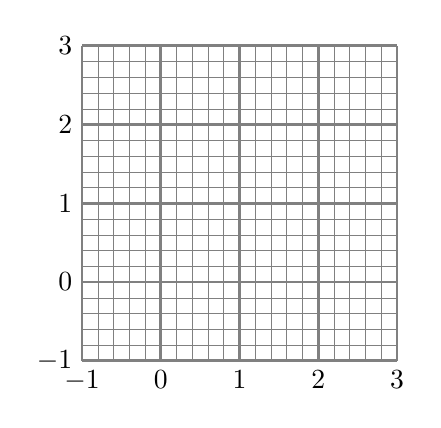
\begin{tikzpicture}

  \draw(-1,-1) to[grid with coordinates,grid with
  coordinates/major line width=1pt] (3,3);

\end{tikzpicture}
\caption{Grid with Coordinates}
\label{fig:grid1}
\end{figure}

The second exame uses the same macro defined before, changing line widths, resulting in \autoref{fig:grid2}

\begin{verbatim}
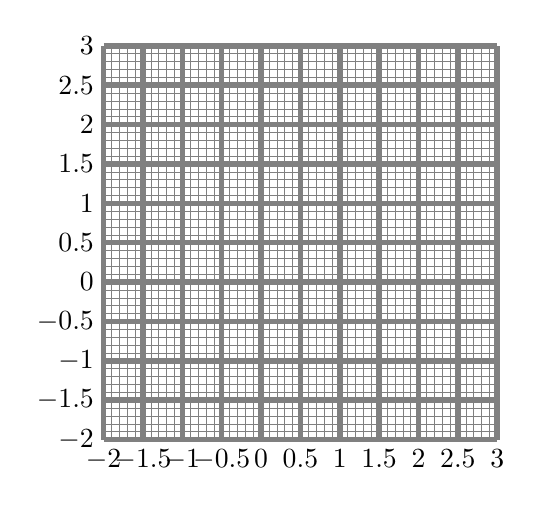
\begin{tikzpicture}

  \draw(-2,-2) to[grid with coordinates,grid with
  coordinates/major line width=2pt,grid with
  coordinates/major step=.5,grid with
  coordinates/minor step=0.1] (3,3);

\end{tikzpicture}
\end{verbatim}

\begin{figure}[hbt]
\centering
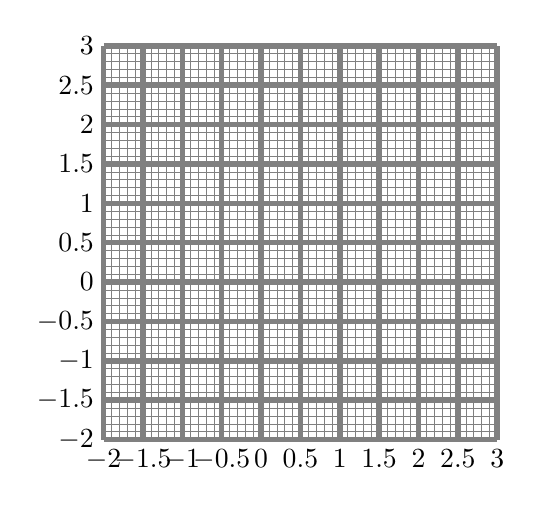
\begin{tikzpicture}

  \draw(-2,-2) to[grid with coordinates,grid with coordinates/major line width=2pt,grid with coordinates/major step=.5,grid with coordinates/minor step=0.1] (3,3);

\end{tikzpicture}
\caption{Grid with Coordinates, another use}
\label{fig:grid2}
\end{figure}

\section{Simple Figures}

\begin{figure}[hbt]
    \centering
    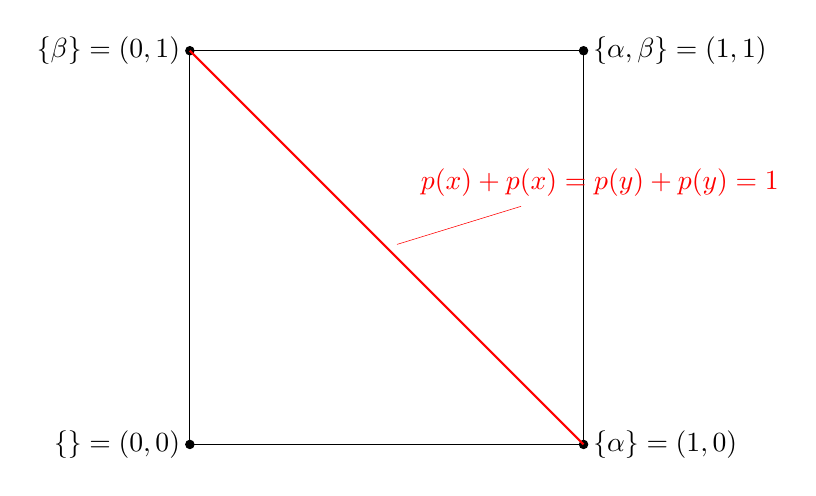
\begin{tikzpicture}
\draw  (0,0)-- (0,5) -- (5,5) -- (5,0) -- (0,0);
\draw[fill=black]  (0,0) circle (1.5pt);
\draw[fill=black]  (5,0) circle (1.5pt);
\draw[fill=black]  (0,5) circle (1.5pt);
\draw[fill=black]  (5,5) circle (1.5pt);
\node[left] at (0,0) {$\{\}=(0,0)$ };
\node[left] at (0,5) {$\{\beta\}=(0,1)$ };
\node[right] at (5,0) {$\{\alpha\}=(1,0)$};
\node[right] at (5,5) {$\{\alpha,\beta\}= (1,1)$};
\draw[color=red,style=thick] (0,5) -- (5,0) node [pin={[pin edge={solid,red}]60:{$p(x)+p(\Bar{x})=p(y)+p(\Bar{y})=1$}},midway] {};

\end{tikzpicture}
    \caption{ERRADA!!!!! }

\end{figure}






\section{Axis and Vectors}



\begin{figure}[hbt]
\centering
\begin{tikzpicture}

% eixos
\draw[very thick,<->] (0,10) -- (0,0) -- (10,0);
\node[rotate=90]
at (-.3,2.5) {$termo_m$};
\node[below] at (2.6,0) {$termo_p$};

% retas verticais
%\draw[dotted] (1,0) -- (1,5);
%\draw[dotted] (2,0) -- (2,5);
%\draw[dotted] (3,0) -- (3,5);
%\draw[dotted] (4,0) -- (4,5);
%\draw[dotted] (5,0) -- (5,5);

% retas horizontais
%\draw[dotted] (0,1) -- (5,1);
%\draw[dotted] (0,2) -- (5,2);
%\draw[dotted] (0,3) -- (5,3);
%\draw[dotted] (0,4) -- (5,4);
%\draw[dotted] (0,5) -- (5,5);



\draw[,[->] (0,0) -- (10,10)  node[above] {$d_1$}  ;

\draw[,red,->] (0,0) -- (5,4)  node[above] {$q$}  ;

\draw[,[->] (0,0) -- (5,1)  node[above] {$d_2$}  ;

\draw[,[->] (0,0) -- (1,5)  node[above] {$d_3$}  ;

\end{tikzpicture}
\caption{Regras fuzzy funcionam como especificação de pedaços das funções sendo agregadas }

\end{figure}
\begin{figure}[hbt]
\centering
\begin{tikzpicture}

% eixos
\draw[very thick,<->] (0,5) -- (0,0) -- (5,0);
\node[rotate=90]
at (-.3,2.5) {$termo_m$};
\node[below] at (2.6,0) {$termo_p$};

\coordinate (origin) at (0,0);
\coordinate (q) at (5,5);
\coordinate (d1) at (5,4);
\coordinate (d2) at (1,4);
\coordinate (d3) at (4,1);


\draw[->] (origin) -- (q)  node[above] {$q$}  ;

\draw[red,->] (origin) -- (d1)  node[above] {$d_1$}  ;

\draw[->,blue] (origin) -- (d2)  node[above] {$d_2$}  ;

\draw[->,orange] (origin) -- (d3)  node[above] {$d_3$}  ;

     \pic [draw,->,"$\alpha$" font=\small,
     angle radius=20mm,orange,
     angle eccentricity=1.1,
     ] {angle=d3--origin--q};

     \pic [draw,->,red,
     angle radius=40mm,
     angle eccentricity=1.1,
     "$\beta$"] {angle=d1--origin--q};

          \pic [draw,->,"$\theta$",
     angle radius=10mm,blue,
     angle eccentricity=1.2,
     ] {angle=q--origin--d2};

\end{tikzpicture}
\caption{Usando o coseno dos vetores. }
\label{fig:cosvet}
\end{figure}

\begin{figure}[hbt]
\centering
\begin{tikzpicture}

% eixos
\draw[very thick,<->] (0,10) -- (0,0) -- (10,0);
\node[rotate=90]
at (-.3,2.5) {$termo_m$};
\node[below] at (2.6,0) {$termo_p$};

\coordinate (origin) at (0,0);
\coordinate (q) at (5,4);
\coordinate (d1) at (10,10);
\coordinate (d2) at (1,4);
\coordinate (d3) at (4,1);


% retas verticais
%\draw[dotted] (1,0) -- (1,5);
%\draw[dotted] (2,0) -- (2,5);
%\draw[dotted] (3,0) -- (3,5);
%\draw[dotted] (4,0) -- (4,5);
%\draw[dotted] (5,0) -- (5,5);

% retas horizontais
%\draw[dotted] (0,1) -- (5,1);
%\draw[dotted] (0,2) -- (5,2);
%\draw[dotted] (0,3) -- (5,3);
%\draw[dotted] (0,4) -- (5,4);
%\draw[dotted] (0,5) -- (5,5);

\draw[->,blue] (origin) -- (d1)  node[above] {$d_1$}  ;
\draw[->] (origin) -- (q)  node[above] {$q$}  ;
\draw[red,->] (origin) -- (d2)  node[above] {$d_2$}  ;
\draw[orange,->] (origin) -- (d3)  node[right] {$d_3$}  ;

\draw[-latex,dashed,blue] (d1) -- (q)  node[label={[label distance=2cm]45:$q-d_1$}] {}  ;
\draw[dashed,red,-latex] (d2) -- (q)  node[label={[label distance=2cm]177:$q-d_2$}] {}  ;
\draw[dashed,orange,-latex] (d3) -- (q) node[label={[label distance=2cm]270:$q-d_3$}] {}  ;



\end{tikzpicture}
\caption{Exemplo de problema com o uso do tamanho dos vetores }
\label{fig:vetdist1}
\end{figure}


\section{Real 3D}

\begin{figure}
\begin{center}
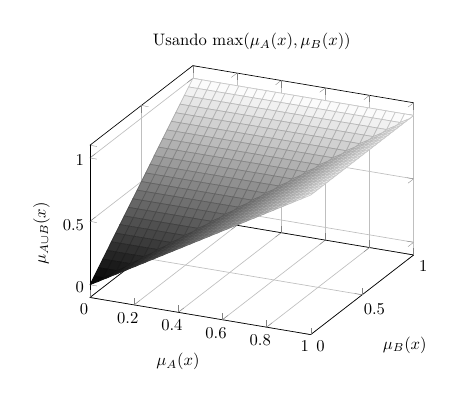
\begin{tikzpicture}[scale=0.6]
  \begin{axis}[grid=both,
  colormap/blackwhite,
  title={Usando $\max(\mu_{\Tilde{A}}(x),\mu_{\Tilde{B}}(x))$},
  xlabel={$\mu_{\Tilde{A}}(x)$},
  ylabel={$\mu_{\Tilde{B}}(x)$},
  zlabel={$\mu_{\Tilde{A}\cup\Tilde{B}}(x)$}
  ]
\addplot3[surf,domain=0:1]
      {max(x,y)};
\end{axis}
\end{tikzpicture}
\qquad
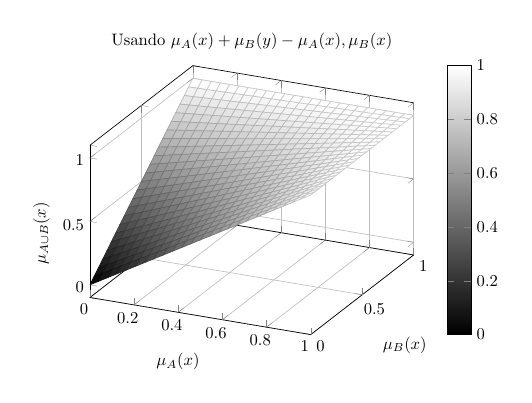
\begin{tikzpicture}[scale=0.6]
  \begin{axis}[grid=both,
    colormap/blackwhite,colorbar,
    title={Usando $\mu_{\Tilde{A}}(x) + \mu_{\Tilde{B}}(y) -
  \mu_{\Tilde{A}}(x),\mu_{\Tilde{B}}(x)$},
  xlabel={$\mu_{\Tilde{A}}(x)$},
  ylabel={$\mu_{\Tilde{B}}(x)$},
  zlabel={$\mu_{\Tilde{A}\cup\Tilde{B}}(x)$}
  ]
    \addplot3[surf,domain=0:1]
      {x+y-x*y)};
  \end{axis}
\end{tikzpicture}
\end{center}
    \caption{Desenho de 3D  (real) a partir de funções.}

\end{figure}

\section{More difficult drawing mixing nodes and curves}



\begin{figure}[hbt]
\centering
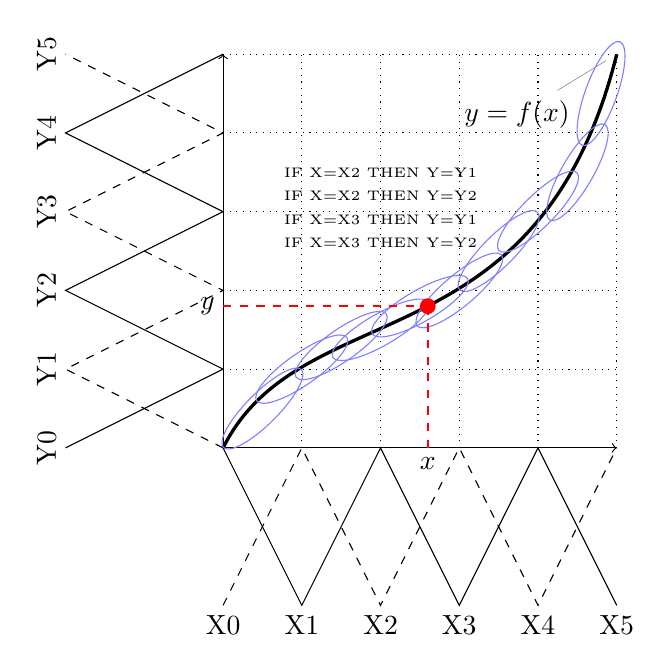
\begin{tikzpicture}

% eixos
\draw[<->] (0,5) -- (0,0) -- (5,0);
\node
at (-.2,1.8) {$y$};
\node[below] at (2.6,0) {$x$};

% triangulos horizontais
\draw (0,0) -- (1,-2) node[below] {X1}-- (2,0) --
        (3,-2) node[below] {X3 }-- (4,0) -- (5,-2) node[below] {X5};
\draw[dashed] (0,-2) node[below] {X0}-- (1,0) -- (2,-2) node[below] {X2} --
        (3,0)-- (4,-2) node[below] {X4} -- (5,0);

% triangulos verticais
\draw (-2,0) node[rotate=90,above] {Y0} -- (0,1) -- (-2,2) node[rotate=90,above] {Y2} --
        (0,3)-- (-2,4) node[rotate=90,above] {Y4} -- (0,5);
\draw[dashed] (0,0) -- (-2,1) node[rotate=90,above] {Y1} -- (0,2) --
        (-2,3) node[rotate=90,above] {Y3} -- (0,4) -- (-2,5) node[rotate=90,above] {Y5};

% retas verticais
\draw[dotted] (1,0) -- (1,5);
\draw[dotted] (2,0) -- (2,5);
\draw[dotted] (3,0) -- (3,5);
\draw[dotted] (4,0) -- (4,5);
\draw[dotted] (5,0) -- (5,5);

% retas horizontais
\draw[dotted] (0,1) -- (5,1);
\draw[dotted] (0,2) -- (5,2);
\draw[dotted] (0,3) -- (5,3);
\draw[dotted] (0,4) -- (5,4);
\draw[dotted] (0,5) -- (5,5);



\draw[very thick] (0,0) coordinate (a1) .. controls  (1,2) and (4,1) .. (5,5) coordinate (a2) node[pin=below left:{$y=f(x)$}] { }  ;

\draw[blue!50,rotate around={45:(0.5,0.5)}] (0.5,0.5) ellipse [x radius=0.7, y radius=0.2];

\draw[blue!50,rotate around={35:(1,1)}] (1,1) ellipse [x radius=0.7, y radius=0.2];

\draw[blue!50,rotate around={35:(1.5,1.3)}] (1.5,1.3) ellipse [x radius=0.7, y radius=0.2];

\draw[blue!50,rotate around={30:(2,1.5)}] (2,1.5) ellipse [x radius=0.7, y radius=0.2];

\draw[blue!50,rotate around={30:(2.5,1.8)}] (2.5,1.8) ellipse [x radius=0.7, y radius=0.2];

\draw[blue!50,rotate around={40:(3,2)}] (3,2) ellipse [x radius=0.7, y radius=0.2];

\draw[blue!50,rotate around={45:(3.5,2.5)}] (3.5,2.5) ellipse [x radius=0.7, y radius=0.2];

\draw[blue!50,rotate around={45:(4,3)}] (4,3) ellipse [x radius=0.7, y radius=0.2];

\draw[blue!50,rotate around={60:(4.5,3.5)}] (4.5,3.5) ellipse [x radius=0.7, y radius=0.2];

\draw[blue!50,rotate around={70:(4.8,4.5)}] (4.8,4.5) ellipse [x radius=0.7, y radius=0.2];

\draw[thick,red,dashed] (2.6,0) -- (2.6,1.8);
\draw[thick,red,dashed] (0,1.8) -- (2.6,1.8);
\fill[red] (2.6,1.8) circle [radius=0.1];

\node[font=\tiny] at (2,3.5) {IF X=X2 THEN Y=Y1};
\node[font=\tiny] at (2,3.2) {IF X=X2 THEN Y=Y2};
\node[font=\tiny] at (2,2.9) {IF X=X3 THEN Y=Y1};
\node[font=\tiny] at (2,2.6) {IF X=X3 THEN Y=Y2};

\end{tikzpicture}
\caption{Regras fuzzy funcionam como especificação de pedaços das funções sendo agregadas }

\end{figure}

\begin{figure}[hbt]
\centering
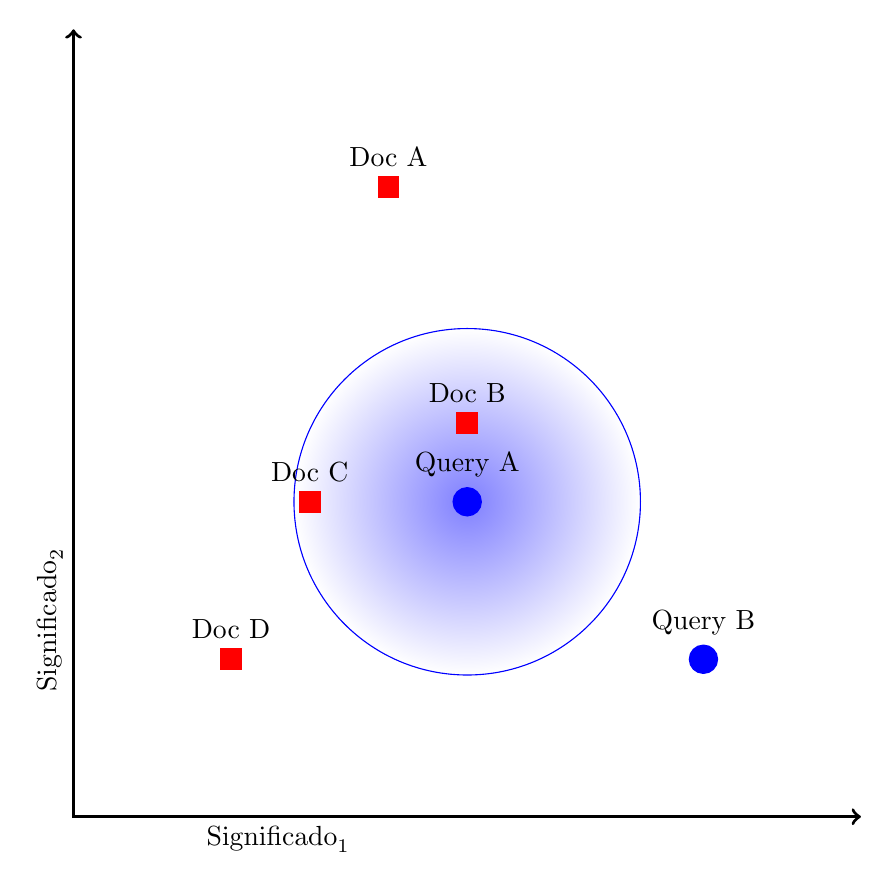
\begin{tikzpicture}[
ponto/.style={rectangle,draw,very thick,color=red,fill=red,
minimum width=5pt,
minimum height=5pt},
query/.style={circle,draw,very thick,color=blue,
minimum width=5pt,fill=blue,
minimum height=5pt}
]

% eixos
\draw[very thick,<->] (0,10) -- (0,0) -- (10,0);
\node[rotate=90]
at (-.3,2.5) {$\textrm{Significado}_2$};
\node[below] at (2.6,0) {$\textrm{Significado}_1$};
\filldraw[even odd rule,inner color=blue!50!white,outer color=white,blue] (5,4) circle (2.2);
\node[ponto,label =above:{Doc D}] at (2,2) {};
\node[ponto,label =above:{Doc A}] at (4,8) {};
%\node[ponto,label =above:{Doc D}] at (6,6) {};
\node[ponto,label =above:{Doc B}] at (5,5) {};
\node[ponto,label =above:{Doc C}] at (3,4) {};
\node[query,label =above:{Query A}] at (5,4) {};
\node[query,label =above:{Query B}] at (8,2) {};


\end{tikzpicture}
\caption{Ideia do Modelo Vetorial}
\label{fig:asdash}
\end{figure}


\begin{figure}[hbt]
\centering
\begin{tikzpicture}

% eixos
\draw[<->] (0,5) -- (0,0) -- (5,0);

% triangulos horizontais
\draw (0,0)
        -- (1,-2) node[below] {X1}
        -- (2,0) ;
\draw[red] (2,0)
        -- (3,-2) node[red,below] {X3 }
        -- (4,0);
\draw   (4,0)
        -- (5,-2) node[below] {X5};

\draw[dashed] (0,-2) node[below] {X0}
        -- (1,0) ;
\draw[blue,dashed] (1,0)
        -- (2,-2) node[below,blue] {X2}
        -- (3,0);
\draw[dashed] (3,0)
        -- (4,-2) node[below] {X4}
        -- (5,0);

% triangulos verticais
\draw (-2,0) node[rotate=90,above] {Y0}
        -- (0,1)
        -- (-2,2) node[red,rotate=90,above] {Y2}
        -- (0,3)
        -- (-2,4) node[rotate=90,above] {Y4}
        -- (0,5);
\draw[dashed] (0,0)
        -- (-2,1) node[rotate=90,above] {Y1}
        -- (0,2)
        -- (-2,3) node[blue,rotate=90,above] {Y3}
        -- (0,4)
        -- (-2,5) node[rotate=90,above] {Y5};

% retas verticais
\draw[dotted] (1,0) -- (1,5);
\draw[dotted] (2,0) -- (2,5);
\draw[dotted] (3,0) -- (3,5);
\draw[dotted] (4,0) -- (4,5);
\draw[dotted] (5,0) -- (5,5);

% retas horizontais
\draw[dotted] (0,1) -- (5,1);
\draw[dotted] (0,2) -- (5,2);
\draw[dotted] (0,3) -- (5,3);
\draw[dotted] (0,4) -- (5,4);
\draw[dotted] (0,5) -- (5,5);



\fill[black] (2.5,0) circle [radius=0.1] node[above] {$x$};
\draw[dotted,->] (2.5,0) -- (2.5,-0.9);
\fill[black] (2.5,-1) circle [radius=0.1] node[right,font=\tiny] {$\mu_{X3}(x)=0.5$};
\node[left,font=\tiny] at (2.5,-1) {$\mu_{X2}(x)=0.5$};

\fill[pattern color=red,pattern=vertical lines] (2,1) rectangle (4,3) ;
\fill[pattern color=blue,pattern=horizontal lines] (1,2) rectangle (3,4) ;

\node[font=\tiny] at (2,4) [above] {IF X=X2 THEN Y=Y3};
\node[font=\tiny] at (3,1) [below] {IF X=X3 THEN Y=Y2};

\fill[pattern color=red,pattern=vertical lines] (0,1) -- (-1,1.5) -- (-1,2.5) -- (0,3);
\fill[pattern color=blue,pattern=horizontal lines] (0,2) -- (-1,2.5) -- (-1,3.5) -- (0,4);

\fill[black] (0,2.5) circle [radius=0.1] node[right] {$y$};


\end{tikzpicture}
    \caption{Duas regras ativadas simultaneamente de um conjunto de regras, a partir de uma entrada $x$, são agregadas e uma função de defuzzificação, como o centróide, é usada para determinar $y$}

\end{figure}



\section{1D}


\begin{figure}[hbt]
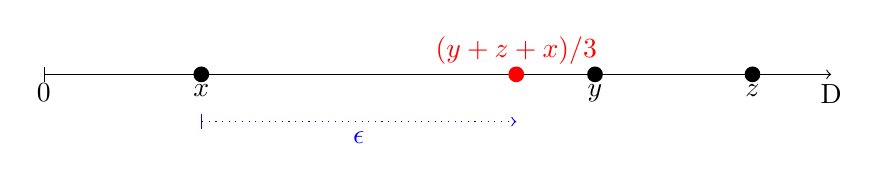
\begin{tikzpicture}
\draw[|->] node[below] {0}  (0,0) -- (10,0)node[below] {D};
\fill[black] (2,0) circle [radius=0.1] node[below] {$x$};
\fill[black] (7,0) circle [radius=0.1] node[below] {$y$};
\fill[black] (9,0) circle [radius=0.1] node[below] {$z$};
\draw[|->,blue,dotted] (2,-0.6) -- (4,-0.6) node[below] {$\epsilon$} -- (6,-0.6);
\fill[red] (6,0)  circle [radius=0.1] node[above] {$(y+z+x)/3$};
\end{tikzpicture}
\caption{Visão gráfica da medida simples de concordância para três pontos, x basicamente em desacordo, considerando um contra a média de todos}

\end{figure}

\begin{figure}[hbt]
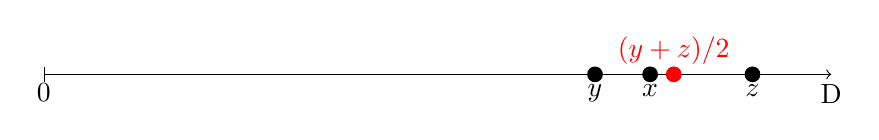
\begin{tikzpicture}
\draw[|->] node[below] {0}  (0,0) -- (10,0)node[below] {D};
\fill[black] (7.7,0) circle [radius=0.1] node[below] {$x$};
\fill[black] (7,0) circle [radius=0.1] node[below] {$y$};
\fill[black] (9,0) circle [radius=0.1] node[below] {$z$};
\fill[red] (8,0)  circle [radius=0.1] node[above] {$(y+z)/2$};
\end{tikzpicture}
\caption{Visão gráfica da medida simples de concordância para três pontos, x basicamente em acordo}

\end{figure}

\section{Desenhos de Fuzzy}



\begin{figure}[hbt]
    \centering
    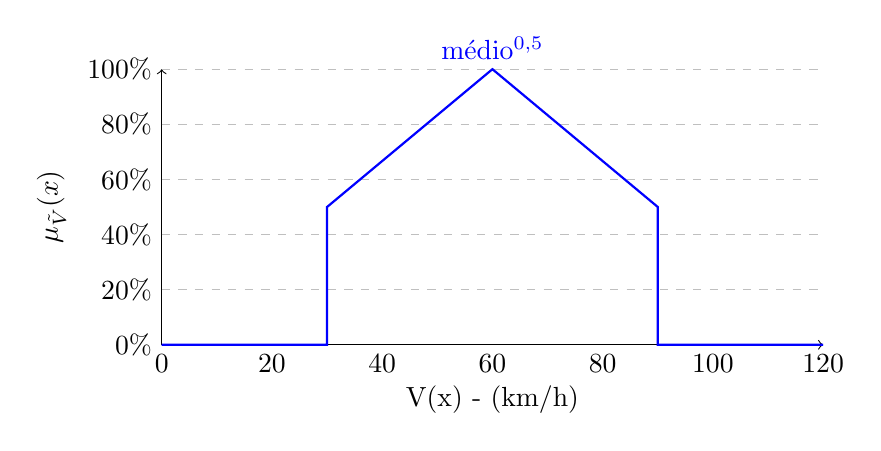
\begin{tikzpicture}[scale=0.7]
\draw[<->] (0,5) -- (0,0) -- (12,0);
\node[left] at (0,5) {$100\%$};
\node[left] at (0,4) {$80\%$};
\node[left] at (0,3) {$60\%$};
\node[left] at (0,2) {$40\%$};
\node[left] at (0,1) {$20\%$};
\node[left] at (0,0) {$0\%$};
\draw[style=dashed,color=gray!50] (0,5) -- (12,5);
\draw[style=dashed,color=gray!50] (0,4) -- (12,4);
\draw[style=dashed,color=gray!50] (0,3) -- (12,3);
\draw[style=dashed,color=gray!50] (0,2) -- (12,2);
\draw[style=dashed,color=gray!50] (0,1) -- (12,1);
\node[below] at (12,0) {$120$};
\node[below] at (10,0) {$100$};
\node[below] at (8,0) {$80$};
\node[below] at (6,0) {$60$};
\node[below] at (4,0) {$40$};
\node[below] at (2,0) {$20$};
\node[below] at (0,0) {$0$};
\draw[color=blue,style=thick] (0,0) -- (3,0) -- (3,2.5) -- (6,5) -- (9,2.5)-- (9,0) -- (12,0);
\node[rotate=90] at (-2,2.5) {$\mu_{\tilde{V}}(x)$};
\node at (6,-1) {V(x) - (km/h)};
\node[above,color=blue]  at (6,5) {médio$^{0,5}$};
\end{tikzpicture}
    \caption{O conjunto referente ao corte-alfa de médio com $\alpha=0,5$, ou seja médio$^{0,5}$.}

\end{figure}

\begin{figure}[hbt]
    \centering
    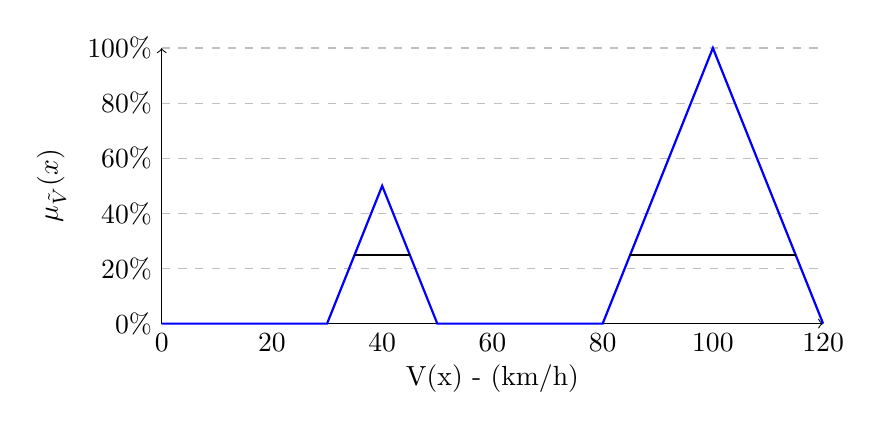
\begin{tikzpicture}[scale=0.7]
\draw[<->] (0,5) -- (0,0) -- (12,0);
\node[left] at (0,5) {$100\%$};
\node[left] at (0,4) {$80\%$};
\node[left] at (0,3) {$60\%$};
\node[left] at (0,2) {$40\%$};
\node[left] at (0,1) {$20\%$};
\node[left] at (0,0) {$0\%$};
\draw[style=dashed,color=gray!50] (0,5) -- (12,5);
\draw[style=dashed,color=gray!50] (0,4) -- (12,4);
\draw[style=dashed,color=gray!50] (0,3) -- (12,3);
\draw[style=dashed,color=gray!50] (0,2) -- (12,2);
\draw[style=dashed,color=gray!50] (0,1) -- (12,1);
\node[below] at (12,0) {$120$};
\node[below] at (10,0) {$100$};
\node[below] at (8,0) {$80$};
\node[below] at (6,0) {$60$};
\node[below] at (4,0) {$40$};
\node[below] at (2,0) {$20$};
\node[below] at (0,0) {$0$};
\node[rotate=90] at (-2,2.5) {$\mu_{\tilde{V}}(x)$};
\node at (6,-1) {V(x) - (km/h)};
\draw[color=blue,style=thick] (0,0) -- (3,0) -- (4,2.5) -- (5,0) -- (8,0)-- (10,5) -- (12,0);
\draw[color=black,style=thick] (3.5,1.25) -- (4.5,1.25);
\draw[color=black,style=thick] (8.5,1.25) -- (11.5,1.25);
\end{tikzpicture}
    \caption{Exemplo de cortes-$\alpha$}

\end{figure}

\begin{figure}[hbt]
    \centering
    \begin{tikzpicture}[yscale=0.05,xscale=.3]
\draw[<->] (0,100) -- (0,0) -- (30,0);
\node[left] at (0,100) {$100\%$};
\node[left] at (0,80) {$80\%$};
\node[left] at (0,60) {$60\%$};
\node[left] at (0,40) {$40\%$};
\node[left] at (0,20) {$20\%$};
\node[left] at (0,0) {$0\%$};
\draw[style=dashed,color=gray!50] (0,100) -- (30,100);
\draw[style=dashed,color=gray!50] (0,80) -- (30,80);
\draw[style=dashed,color=gray!50] (0,60) -- (30,60);
\draw[style=dashed,color=gray!50] (0,40) -- (30,40);
\draw[style=dashed,color=gray!50] (0,20) -- (30,20);
\node[below] at (30,0) {$30$};
\node[below] at (25,0) {$25$};
\node[below] at (20,0) {$20$};
\node[below] at (15,0) {$15$};
\node[below] at (10,0) {$10$};
\node[below] at (5,0) {$5$};
\node[below] at (0,0) {$0$};

\draw[color=black,style=thick] (3,20) -- (11,20);
\draw[color=black,style=thick] (16,20) -- (24,20);

\draw[color=black,style=thick] (4,40) -- (10,40);
\draw[color=black,style=thick] (17,40) -- (23,40);

\draw[color=black,style=thick] (5,60) -- (9,60);
\draw[color=black,style=thick] (18,60) -- (22,60);

\draw[color=black,style=thick] (6,80) -- (8,80);
\draw[color=black,style=thick] (19,80) -- (21,80);

\node[rotate=90] at (-5,50) {$\mu_{\tilde{A}}(x)$};

\node at (15,-15) {x};

\end{tikzpicture}
    \caption{Representação dos cortes-$\alpha$ do conjunto $\tilde{A}$ dos números perto de 7 ou 20}

\end{figure}



\begin{figure}[hbt]
\centering
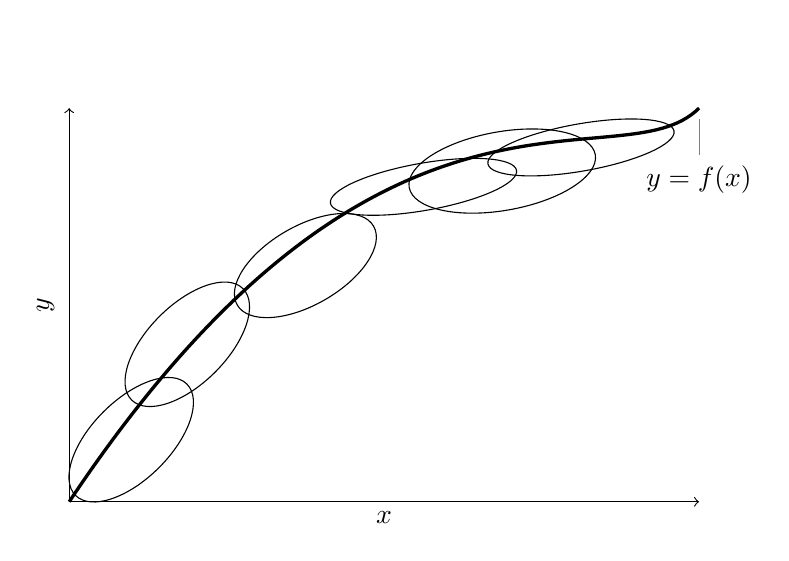
\begin{tikzpicture}
\draw[<->] (0,5) -- (0,0) -- (8,0);
\node[rotate=90] at (-.3,2.5) {$y$};
\node[below] at (4,0) {$x$};

\draw[very thick] (0,0) .. controls (4,6) and (7,4).. (8,5) node[pin=below:{$y=f(x)$}] { } ;
\draw[rotate around={45:(1,1)}] (0.7,1)ellipse [x radius=1, y radius=0.5];
\draw[rotate around={45:(1.5,2)}] (1.5,2)ellipse [x radius=1, y radius=0.5];
\draw[rotate around={30:(3,3)}] (3,3)ellipse [x radius=1, y radius=0.5];
\draw[rotate around={10:(4.5,4)}] (4.5,4)ellipse [x radius=1.2, y radius=0.3];
\draw[rotate around={10:(5.5,4.2)}] (5.5,4.2)ellipse [x radius=1.2, y radius=0.5];
\draw[rotate around={10:(6.5,4.5)}] (6.5,4.5)ellipse [x radius=1.2, y radius=0.3];
 \end{tikzpicture}
 \caption{Grafico de $y=f(x)$}
\end{figure}





\begin{figure}
\centering

\begin{tikzpicture}[scale=0.7]

\def\pttocm#1{\pgfmathparse{#1 / 19.93333
    }\pgfmathprintnumber{\pgfmathresult}}

    \newcommand{\printcoords}[1]{
      \newdimen\posx
      \pgfextractx{\posx}{\pgfpointanchor{#1}{center}}
      \newdimen\posy
      \pgfextracty{\posy}{\pgfpointanchor{#1}{center}}
      (\pttocm\posx ; \pttocm\posy )
    }


\draw[<->] (0,5) -- (0,0) -- (12,0);
\node[left] at (0,5) {$100\%$};
\node[left] at (0,4) {$80\%$};
\node[left] at (0,3) {$60\%$};
\node[left] at (0,2) {$40\%$};
\node[left] at (0,1) {$20\%$};
\node[left] at (0,0) {$0\%$};
\draw[style=dashed,color=gray!50] (0,5) -- (12,5);
\draw[style=dashed,color=gray!50] (0,4) -- (12,4);
\draw[style=dashed,color=gray!50] (0,3) -- (12,3);
\draw[style=dashed,color=gray!50] (0,2) -- (12,2);
\draw[style=dashed,color=gray!50] (0,1) -- (12,1);
\node[below] at (12,0) {$120$};
\node[below] at (10,0) {$100$};
\node[below] at (8,0) {$80$};
\node[below] at (6,0) {$60$};
\node[below] at (4,0) {$40$};
\node[below] at (2,0) {$20$};
\node[below] at (0,0) {$0$};
\draw[color=blue,style=thick,style=dotted,name path=vava] (0,0) -- (3,0) -- (4,2.5) -- (5,0) -- (8,0)-- (10,5) node[above] {$\Tilde{A}$} -- (12,0);
\path[name path=xixi,draw=none] (0,1) -- (12,1);
\path[name intersections={of=vava and xixi }];
\coordinate (A) at (intersection-1);
\coordinate (B) at (intersection-2);
\coordinate (C) at (intersection-3);
\coordinate (D) at (intersection-4);
\draw[color=black,style=thick] (A) node[left] {\printcoords{A}} -- (B);
\draw[color=black,style=thick] (C) --  (D) node[right] {$\tilde{A}^{20\%}$}  ;
\path[name path=xuxu,draw=none] (0,2) -- (12,2);
\path[name intersections={of=vava and xuxu }];
\coordinate (A) at (intersection-1);
\coordinate (B) at (intersection-2);
\coordinate (C) at (intersection-3);
\coordinate (D) at (intersection-4);
\draw[color=red,style=thick] (A) -- (B);
\draw[color=red,style=thick] (C) -- (D) node[right] {$\Tilde{A}^{40\%}$};
\path[name path=xexe,draw=none] (0,3) -- (12,3);
\path[name intersections={of=vava and xexe }];
\coordinate (A) at (intersection-1);
\coordinate (B) at (intersection-2);
\draw[color=green,style=thick] (A) -- (B) node[right] {$\Tilde{A}^{60\%}$};
\path[name path=xaxa,draw=none] (0,4) -- (12,4);
\path[name intersections={of=vava and xaxa }];
\coordinate (A) at (intersection-1);
\coordinate (B) at (intersection-2);
\draw[color=orange,style=thick] (A) -- (B)node[right] {$\Tilde{A}^{80\%}$};
\end{tikzpicture}
    \caption{Exemplo de cortes-$\alpha$, onde as linhas horizontais indicam os valores do eixo das abcissas que pertencem ao conjunto nítido correspondente}

\end{figure}


\section{Gráficos a partir de números}
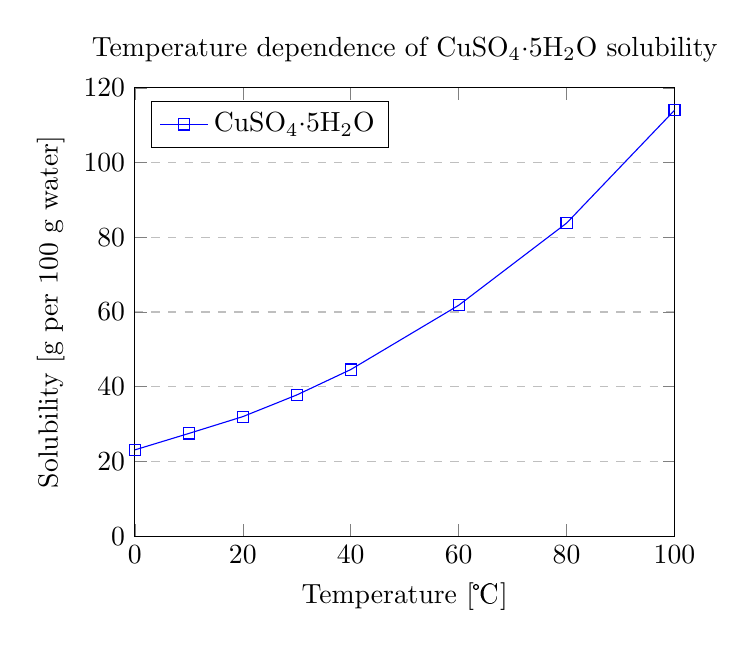
\begin{tikzpicture}
\begin{axis}[
    title={Temperature dependence of CuSO\(_4\cdot\)5H\(_2\)O solubility},
    xlabel={Temperature [\textcelsius]},
    ylabel={Solubility [g per 100 g water]},
    xmin=0, xmax=100,
    ymin=0, ymax=120,
    xtick={0,20,40,60,80,100},
    ytick={0,20,40,60,80,100,120},
    legend pos=north west,
    ymajorgrids=true,
    grid style=dashed,
]

\addplot[
    color=blue,
    mark=square,
    ]
    coordinates {
    (0,23.1)(10,27.5)(20,32)(30,37.8)(40,44.6)(60,61.8)(80,83.8)(100,114)
    };
    \legend{CuSO\(_4\cdot\)5H\(_2\)O}

\end{axis}
\end{tikzpicture}

\begin{tikzpicture}
\draw[<->] (0,11) -- (0,0) -- (11,0);

\foreach \i in {0,1,...,10} \draw (\i,0)--(\i,-.1);
\foreach \i in {0,.2,...,1} \node[below] at (10*\i,0) {\pgfmathprintnumber
[fixed,fixed zerofill,precision=1,use comma]
{\i}};
\node[below] at (5.5,-.5) {Revocação};

\foreach \i in {0,1,...,10} \draw (0,\i)--(-.1,\i);
\foreach \i in {0,.2,...,1} \node[left] at (0,10*\i) {\pgfmathprintnumber
[fixed,fixed zerofill,precision=1,use comma]
{\i}};
\node[rotate=90] at (-.8,5.5) {Precisão};

\draw[very thick] (1,10) ..
controls (8,9)  and    (3,0)
.. (10,1) ;

\node at (4,10) {Consultas específicas};
\node at (9,2) {Consultas genéricas};


\end{tikzpicture}